% =============================================================================
% DREAM paper — LaTeX include snippets for all figures and tables.
% Source scripts: figures/scripts/gen_*.py + this file.
% Place this file under figures/paper/ and \input each block from main.tex.
% =============================================================================

% --- Fig 1: Hero (2-panel) --------------------------------------------------
\begin{figure*}[t]
    \centering
    \begin{subfigure}[t]{0.49\textwidth}
        \centering
        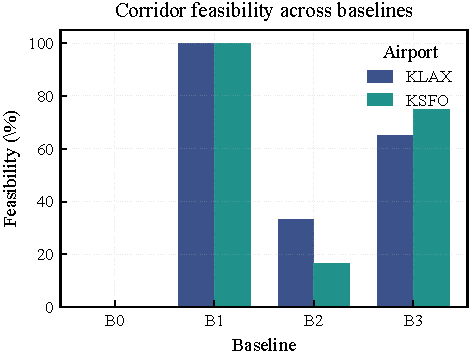
\includegraphics[width=\linewidth]{figures/paper/fig_feasibility_by_baseline.pdf}
        \caption{Per-baseline corridor feasibility.}
        \label{fig:feas-bar}
    \end{subfigure}\hfill
    \begin{subfigure}[t]{0.49\textwidth}
        \centering
        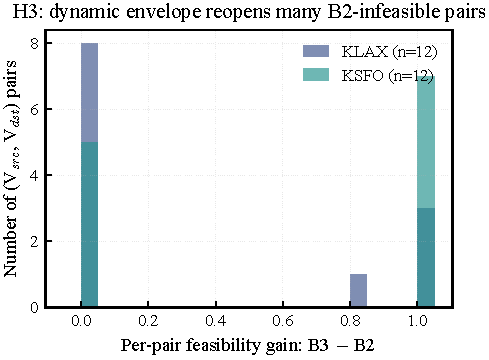
\includegraphics[width=\linewidth]{figures/paper/fig_h3_b2_vs_b3.pdf}
        \caption{Per-pair B3 $-$ B2 feasibility gain.}
        \label{fig:h3-hist}
    \end{subfigure}
    \caption{\textbf{Headline result.} The runway-configuration-aware dynamic envelope (B3)
        recovers \textbf{2.0$\times$ of LAX} and \textbf{4.5$\times$ of SFO} vertiport-pair feasibility
        that the static Annex 14 both-sides-closed baseline (B2) pessimistically forbids,
        on real ADS-B from 5 Aug-2024 Fridays at each airport.}
    \label{fig:hero}
\end{figure*}

% --- Fig 2: System diagram (TikZ, full-width) -------------------------------
% Fig 2 — DREAM system diagram (TikZ skeleton).
%
% Manual draw element — refine line widths, fonts, and labels in final paper.
% Designed as full-width (0.95\textwidth) horizontal flow with 6 boxes + arrows.
%
% Compile in the main paper with:  % Fig 2 — DREAM system diagram (TikZ skeleton).
%
% Manual draw element — refine line widths, fonts, and labels in final paper.
% Designed as full-width (0.95\textwidth) horizontal flow with 6 boxes + arrows.
%
% Compile in the main paper with:  % Fig 2 — DREAM system diagram (TikZ skeleton).
%
% Manual draw element — refine line widths, fonts, and labels in final paper.
% Designed as full-width (0.95\textwidth) horizontal flow with 6 boxes + arrows.
%
% Compile in the main paper with:  \input{figures/paper/fig2_system_diagram.tex}
%
\begin{figure*}[t]
\centering
\begin{tikzpicture}[
    node distance=14mm and 8mm,
    box/.style={
        rectangle, rounded corners, draw, fill=gray!8,
        minimum width=23mm, minimum height=14mm,
        font=\small, align=center,
    },
    src/.style={box, fill=blue!8, draw=blue!50!black},
    out/.style={box, fill=green!8, draw=green!50!black},
    arr/.style={-{Latex[length=2mm]}, semithick},
]
% Row of 6 lanes
\node[src]                  (data)  {Data lane\\\footnotesize FAA · USGS · OSM\\\footnotesize adsb.lol · METAR};
\node[box, right=of data]   (geom)  {Geometry\\\footnotesize OLS $\to$ 3-D SDF\\\footnotesize Vertiport OFV};
\node[box, right=of geom]   (traf)  {Traffic\\\footnotesize Runway-config\\\footnotesize Dynamic envelope};
\node[box, right=of traf]   (ml)    {ML\\\footnotesize Counterfactual\\\footnotesize XGB + conformal};
\node[box, right=of ml]     (plan)  {Planning\\\footnotesize Envelope-aware A*\\\footnotesize 5-term cost};
\node[out, right=of plan]   (eval)  {Analysis\\\footnotesize Safety / Capacity\\\footnotesize / Accessibility KPI};

% Top-row inputs to geometry + traffic + ml
\draw[arr] (data) -- (geom);
\draw[arr] (data.east) to[bend right=12] (traf.west);
\draw[arr] (data.east) to[bend right=22] (ml.west);

\draw[arr] (geom) -- (traf);
\draw[arr] (geom.east) to[bend right=12] (ml.west);
\draw[arr] (geom.east) to[bend right=22] (plan.west);

\draw[arr] (traf) -- (ml);
\draw[arr] (traf.east) to[bend right=12] (plan.west);

\draw[arr] (ml)   -- (plan);
\draw[arr] (plan) -- (eval);

% Footer label
\node[font=\footnotesize, below=4mm of plan.south] (capnote)
    {DREAM pipeline. All lanes ship a \texttt{sanity\_check} entry-point exercised by \texttt{scripts/run\_sanity.py}.};
\end{tikzpicture}
\caption{DREAM framework lanes. Real airport / ADS-B / weather data flow through
    six lanes culminating in safety/capacity/accessibility KPIs. The geometry
    lane encodes ICAO Annex~14 as a 3-D signed-distance field; the traffic lane
    converts ADS-B into a runway-configuration-aware dynamic envelope; the ML
    lane learns a risk field by counterfactual injection; planning runs an
    envelope-constrained A* over a 5-term cost.}
\label{fig:dream-pipeline}
\end{figure*}

%
\begin{figure*}[t]
\centering
\begin{tikzpicture}[
    node distance=14mm and 8mm,
    box/.style={
        rectangle, rounded corners, draw, fill=gray!8,
        minimum width=23mm, minimum height=14mm,
        font=\small, align=center,
    },
    src/.style={box, fill=blue!8, draw=blue!50!black},
    out/.style={box, fill=green!8, draw=green!50!black},
    arr/.style={-{Latex[length=2mm]}, semithick},
]
% Row of 6 lanes
\node[src]                  (data)  {Data lane\\\footnotesize FAA · USGS · OSM\\\footnotesize adsb.lol · METAR};
\node[box, right=of data]   (geom)  {Geometry\\\footnotesize OLS $\to$ 3-D SDF\\\footnotesize Vertiport OFV};
\node[box, right=of geom]   (traf)  {Traffic\\\footnotesize Runway-config\\\footnotesize Dynamic envelope};
\node[box, right=of traf]   (ml)    {ML\\\footnotesize Counterfactual\\\footnotesize XGB + conformal};
\node[box, right=of ml]     (plan)  {Planning\\\footnotesize Envelope-aware A*\\\footnotesize 5-term cost};
\node[out, right=of plan]   (eval)  {Analysis\\\footnotesize Safety / Capacity\\\footnotesize / Accessibility KPI};

% Top-row inputs to geometry + traffic + ml
\draw[arr] (data) -- (geom);
\draw[arr] (data.east) to[bend right=12] (traf.west);
\draw[arr] (data.east) to[bend right=22] (ml.west);

\draw[arr] (geom) -- (traf);
\draw[arr] (geom.east) to[bend right=12] (ml.west);
\draw[arr] (geom.east) to[bend right=22] (plan.west);

\draw[arr] (traf) -- (ml);
\draw[arr] (traf.east) to[bend right=12] (plan.west);

\draw[arr] (ml)   -- (plan);
\draw[arr] (plan) -- (eval);

% Footer label
\node[font=\footnotesize, below=4mm of plan.south] (capnote)
    {DREAM pipeline. All lanes ship a \texttt{sanity\_check} entry-point exercised by \texttt{scripts/run\_sanity.py}.};
\end{tikzpicture}
\caption{DREAM framework lanes. Real airport / ADS-B / weather data flow through
    six lanes culminating in safety/capacity/accessibility KPIs. The geometry
    lane encodes ICAO Annex~14 as a 3-D signed-distance field; the traffic lane
    converts ADS-B into a runway-configuration-aware dynamic envelope; the ML
    lane learns a risk field by counterfactual injection; planning runs an
    envelope-constrained A* over a 5-term cost.}
\label{fig:dream-pipeline}
\end{figure*}

%
\begin{figure*}[t]
\centering
\begin{tikzpicture}[
    node distance=14mm and 8mm,
    box/.style={
        rectangle, rounded corners, draw, fill=gray!8,
        minimum width=23mm, minimum height=14mm,
        font=\small, align=center,
    },
    src/.style={box, fill=blue!8, draw=blue!50!black},
    out/.style={box, fill=green!8, draw=green!50!black},
    arr/.style={-{Latex[length=2mm]}, semithick},
]
% Row of 6 lanes
\node[src]                  (data)  {Data lane\\\footnotesize FAA · USGS · OSM\\\footnotesize adsb.lol · METAR};
\node[box, right=of data]   (geom)  {Geometry\\\footnotesize OLS $\to$ 3-D SDF\\\footnotesize Vertiport OFV};
\node[box, right=of geom]   (traf)  {Traffic\\\footnotesize Runway-config\\\footnotesize Dynamic envelope};
\node[box, right=of traf]   (ml)    {ML\\\footnotesize Counterfactual\\\footnotesize XGB + conformal};
\node[box, right=of ml]     (plan)  {Planning\\\footnotesize Envelope-aware A*\\\footnotesize 5-term cost};
\node[out, right=of plan]   (eval)  {Analysis\\\footnotesize Safety / Capacity\\\footnotesize / Accessibility KPI};

% Top-row inputs to geometry + traffic + ml
\draw[arr] (data) -- (geom);
\draw[arr] (data.east) to[bend right=12] (traf.west);
\draw[arr] (data.east) to[bend right=22] (ml.west);

\draw[arr] (geom) -- (traf);
\draw[arr] (geom.east) to[bend right=12] (ml.west);
\draw[arr] (geom.east) to[bend right=22] (plan.west);

\draw[arr] (traf) -- (ml);
\draw[arr] (traf.east) to[bend right=12] (plan.west);

\draw[arr] (ml)   -- (plan);
\draw[arr] (plan) -- (eval);

% Footer label
\node[font=\footnotesize, below=4mm of plan.south] (capnote)
    {DREAM pipeline. All lanes ship a \texttt{sanity\_check} entry-point exercised by \texttt{scripts/run\_sanity.py}.};
\end{tikzpicture}
\caption{DREAM framework lanes. Real airport / ADS-B / weather data flow through
    six lanes culminating in safety/capacity/accessibility KPIs. The geometry
    lane encodes ICAO Annex~14 as a 3-D signed-distance field; the traffic lane
    converts ADS-B into a runway-configuration-aware dynamic envelope; the ML
    lane learns a risk field by counterfactual injection; planning runs an
    envelope-constrained A* over a 5-term cost.}
\label{fig:dream-pipeline}
\end{figure*}


% --- Fig 3: 3-D OLS rendering for LAX ---------------------------------------
\begin{figure}[t]
    \centering
    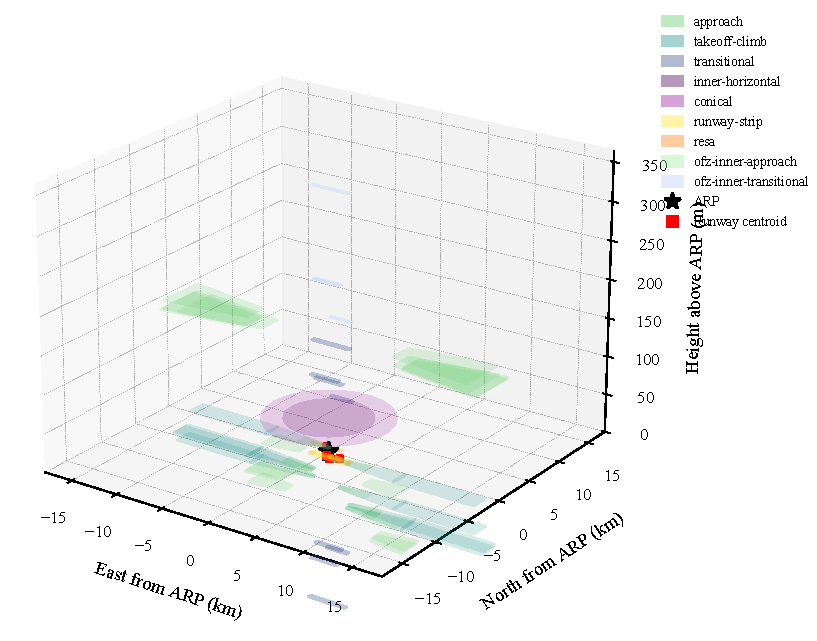
\includegraphics[width=\linewidth]{figures/paper/fig3_ols_3d_klax.pdf}
    \caption{Annex 14 OLS for LAX (KLAX), as 98 prisms rendered at their
        top-of-prism polygons. Approach, takeoff-climb, transitional,
        inner-horizontal, conical, runway-strip, RESA, and OFZ surfaces are
        coloured per family. ARP marked $\star$; runway centroids in red.}
    \label{fig:ols-3d}
\end{figure}

% --- Fig 4: Dynamic envelope filmstrip --------------------------------------
\begin{figure*}[t]
    \centering
    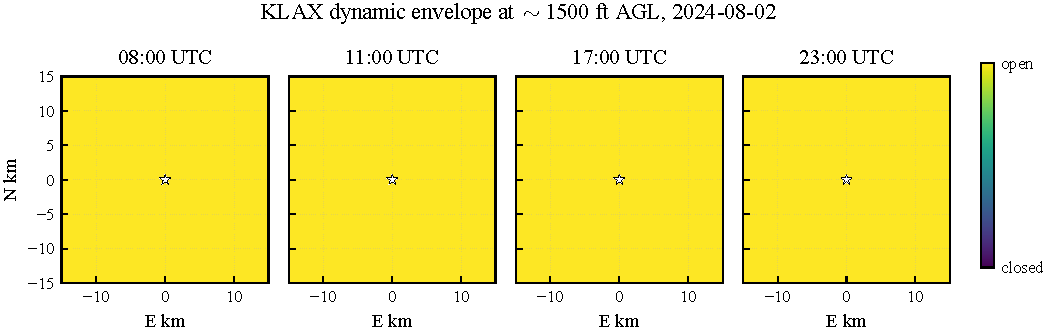
\includegraphics[width=\linewidth]{figures/paper/fig4_envelope_filmstrip_klax.pdf}
    \caption{LAX dynamic envelope at $\sim$1500 ft AGL on 2024-08-02 at four UTC
        hours. Yellow = open for eVTOL traffic, purple = closed by the
        runway-configuration-aware envelope $\mathcal{E}_t$. The closure pattern
        rotates with the active runway configuration inferred from real ADS-B.}
    \label{fig:envelope-filmstrip}
\end{figure*}

% --- Fig 5: Risk-field AUROC -------------------------------------------------
\begin{figure}[t]
    \centering
    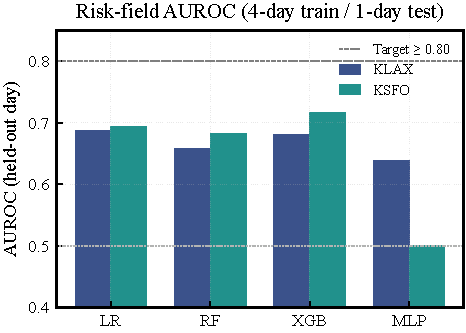
\includegraphics[width=\linewidth]{figures/paper/fig_xgb_metrics.pdf}
    \caption{Risk-field AUROC on the temporally held-out test day (2024-08-30),
        4-day train (08-02/09/16/23) per airport. LR, RF, and XGB cluster within
        $\pm 0.05$ at both airports, indicating a feature ceiling rather than a
        model-class ceiling.}
    \label{fig:xgb}
\end{figure}

% --- Fig 6: Corridor length boxplot -----------------------------------------
\begin{figure}[t]
    \centering
    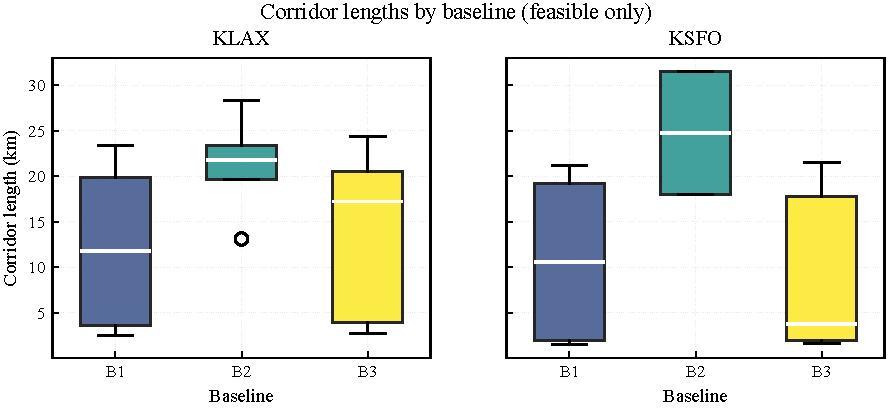
\includegraphics[width=\linewidth]{figures/paper/fig_length_per_baseline.pdf}
    \caption{Corridor length (km) per baseline at LAX and SFO. Conditioned on
        feasibility — only feasible corridors enter. B3 grows path length by
        $\leq 20\%$ over B1 straight lines, in exchange for the
        $\mathcal{E}_t$-respecting safety.}
    \label{fig:length}
\end{figure}

% --- Fig 7: Vertiport-pair feasibility heatmaps -----------------------------
\begin{figure*}[t]
    \centering
    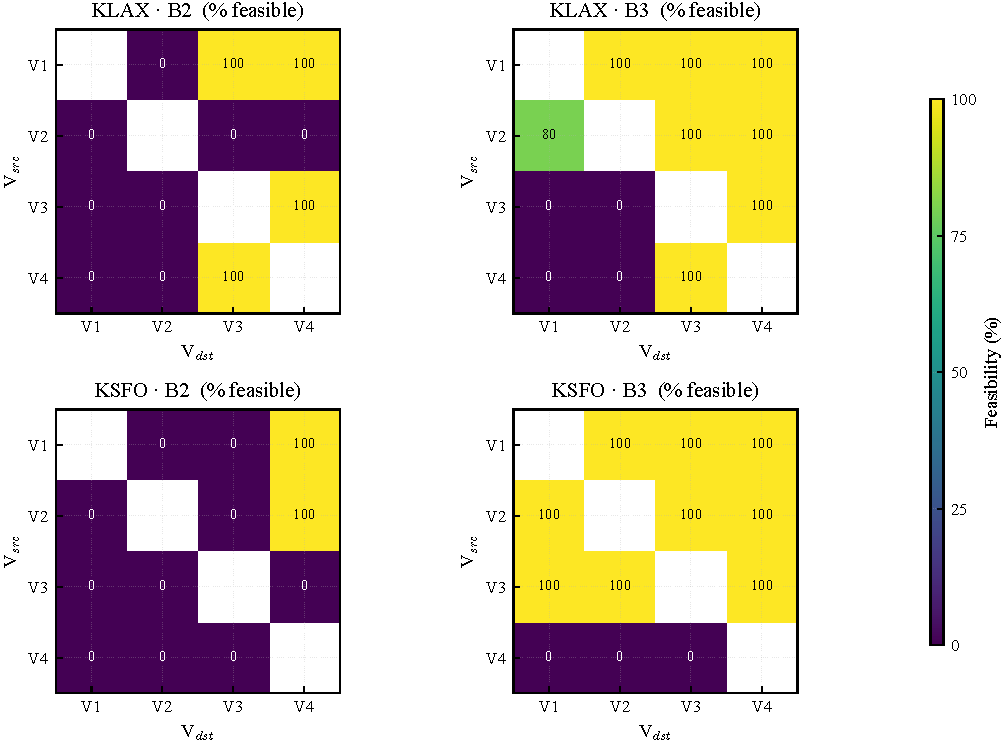
\includegraphics[width=0.85\linewidth]{figures/paper/fig7_vertiport_heatmap.pdf}
    \caption{Per-vertiport-pair feasibility (\%) under B2 (left) and B3 (right)
        at LAX (top) and SFO (bottom). Rows / columns are the four candidate
        vertiport classes (V1 off-fence, V2 landside, V3 rooftop, V4 city-end).
        B3 lifts the V3-rooftop column substantially at both airports —
        operational support for H3 (\S\ref{sec:discussion}).}
    \label{fig:vertiport-heatmap}
\end{figure*}

% --- Table 1: Headline KPI table --------------------------------------------
\begin{table}[t]
\centering
\caption{Real-data DREAM headline. Per-baseline corridor counts ($n=180$), feasibility (\%, fraction of 12 vertiport pairs $\times$ 3 hours $\times$ 5 Aug-2024 Fridays that the planner returns a feasible corridor for), mean corridor length (km, over feasible only), and mean A* expansions.}
\label{tab:headline}
\begin{tabular}{lrrrrrrrr}
\toprule
 & \multicolumn{4}{c}{LAX (KLAX)} & \multicolumn{4}{c}{SFO (KSFO)} \\
\cmidrule(lr){2-5} \cmidrule(lr){6-9}
Baseline & $n$ & feas.\% & len.\,km & pops & $n$ & feas.\% & len.\,km & pops \\
\midrule
B0 & 180 & 0.0 & — & 0 & 180 & 0.0 & — & 0 \\
B1 & 180 & 100.0 & 12.2 & 0 & 180 & 100.0 & 10.9 & 0 \\
B2 & 180 & 33.3 & 21.2 & 16032 & 180 & 16.7 & 24.7 & 10204 \\
B3 & 180 & 65.0 & 13.1 & 9498 & 180 & 75.0 & 8.2 & 4775 \\
\midrule
\multicolumn{9}{l}{\footnotesize B3 vs B2 feasibility lift: \textbf{2.0$\times$} LAX, \textbf{4.5$\times$} SFO.} \\
\bottomrule
\end{tabular}
\end{table}


% --- Table 2: Per-day data manifest -----------------------------------------
\begin{table}[t]
\centering
\caption{Real-data ADS-B inventory per Friday in August 2024, acquired from the open \texttt{adsb.lol} historical archive. Within a 30 NM ARP-centred bounding box. Note the $\sim$50\% coverage drop after 2024-08-09 at both airports, reflecting fewer volunteer receivers on the later Fridays.}
\label{tab:data}
\begin{tabular}{lrrrrrr}
\toprule
 & \multicolumn{3}{c}{LAX (KLAX)} & \multicolumn{3}{c}{SFO (KSFO)} \\
\cmidrule(lr){2-4}\cmidrule(lr){5-7}
Date (Fri) & rows & a/c & MB & rows & a/c & MB \\
\midrule
2024-08-02 & 1,124,625 & 3,763 & 31.0 & 851,836 & 2,069 & 21.8 \\
2024-08-09 & 1,144,920 & 3,851 & 31.8 & 826,573 & 2,084 & 21.1 \\
2024-08-16 & 565,660 & 1,834 & 16.1 & 404,611 & 1,004 & 11.4 \\
2024-08-23 & 498,990 & 1,632 & 14.5 & 366,808 & 899 & 10.4 \\
2024-08-30 & 456,486 & 1,523 & 13.4 & 342,184 & 865 & 9.9 \\
\midrule
\textbf{Sum} & \textbf{3,790,681} & & & \textbf{2,792,012} & & \\
\bottomrule
\end{tabular}
\end{table}


% --- Table 3: Risk-field model comparison -----------------------------------
\begin{table}[t]
\centering
\caption{Real-data risk-field models. 4 Aug-2024 Fridays $\rightarrow$ 1 Friday temporal holdout. $n_{\textrm{train}}=180\,000$, $n_{\textrm{test}}=40\,000$ counterfactual eVTOL segments. \emph{Conformal coverage} is the empirical hit rate of the split-conformal 90\,\% prediction interval; target window $0.88$--$0.92$ is shown in \textbf{bold} on rows that hit it. AUROC clusters within $\pm 0.05$ across LR/RF/XGB at both airports, indicating a feature ceiling — discussed in \S\ref{sec:discussion}.}
\label{tab:risk}
\begin{tabular}{llrrr rr}
\toprule
Airport & Model & AUROC & AUPR & Conformal cov. & pos$_{\textrm{tr}}$ & pos$_{\textrm{te}}$ \\
\midrule
KLAX & LR & 0.687 & 0.570 & 0.864 & 0.57 & 0.41 \\
KLAX & RF & 0.659 & 0.527 & 0.940 & 0.57 & 0.41 \\
KLAX & XGB & 0.680 & 0.564 & 0.780 & 0.57 & 0.41 \\
KLAX & MLP & 0.639 & 0.527 & 1.000 & 0.57 & 0.41 \\
\midrule
KSFO & LR & 0.695 & 0.377 & 0.936 & 0.35 & 0.21 \\
KSFO & RF & 0.682 & 0.314 & 0.962 & 0.35 & 0.21 \\
KSFO & \textbf{XGB} & 0.716 & 0.402 & \textbf{0.912} & 0.35 & 0.21 \\
KSFO & MLP & 0.500 & 0.212 & 1.000 & 0.35 & 0.21 \\
\bottomrule
\end{tabular}
\end{table}


% --- Table 4: Annex 14 parameters -------------------------------------------
\begin{table}[t]
\centering
\caption{Annex 14 OLS parameters used by DREAM (generic Code 4 precision approach). These are public-secondary-source placeholder values, not a copy of the ICAO normative text. Per-airport calibration is supported via the YAML override in \texttt{configs/annex14/}.}
\label{tab:ols-params}
\begin{tabular}{lr}
\toprule
Parameter & Value \\
\midrule
Approach surface (inner edge / divergence) & 300 m / 0.150 rad \\
Approach section 1 (slope $\times$ length) & 1:50 $\times$ 3000 m \\
Approach section 2 (slope $\times$ length) & 1:40 $\times$ 3600 m \\
Takeoff-climb (slope $\times$ length) & 1:50 $\times$ 15000 m \\
Transitional slope & 1:7 \\
Inner horizontal (radius / height) & 4000 m / 45 m \\
Conical (slope / height) & 1:20 / 100 m \\
Runway strip (half-width / end length) & 150 m / 60 m \\
Runway end safety area (RESA) & 240 $\times$ 150 m \\
OFZ inner-approach (slope $\times$ length) & 1:50 $\times$ 900 m \\
OFZ inner-transitional slope & 1:3 \\
Vertiport approach/departure (slope, FAA EB-105A) & 1:8 \\
Vertiport OFV (FATO half-side / height) & 16 m / 300 m \\
\bottomrule
\end{tabular}
\end{table}

